\documentclass{standalone}
\usepackage{graphicx}	
\usepackage{amssymb, amsmath}
\usepackage{color}

\usepackage{tikz}
\usetikzlibrary{intersections, backgrounds}
\usepackage{pgfmath}

\definecolor{light}{RGB}{220, 188, 188}
\definecolor{mid}{RGB}{185, 124, 124}
\definecolor{dark}{RGB}{143, 39, 39}
\definecolor{highlight}{RGB}{180, 31, 180}
\definecolor{gray10}{gray}{0.1}
\definecolor{gray20}{gray}{0.2}
\definecolor{gray30}{gray}{0.3}
\definecolor{gray40}{gray}{0.4}
\definecolor{gray60}{gray}{0.6}
\definecolor{gray70}{gray}{0.7}
\definecolor{gray80}{gray}{0.8}
\definecolor{gray90}{gray}{0.9}
\definecolor{gray95}{gray}{0.95}

\newcommand*{\offset}{0.025}

\begin{document}

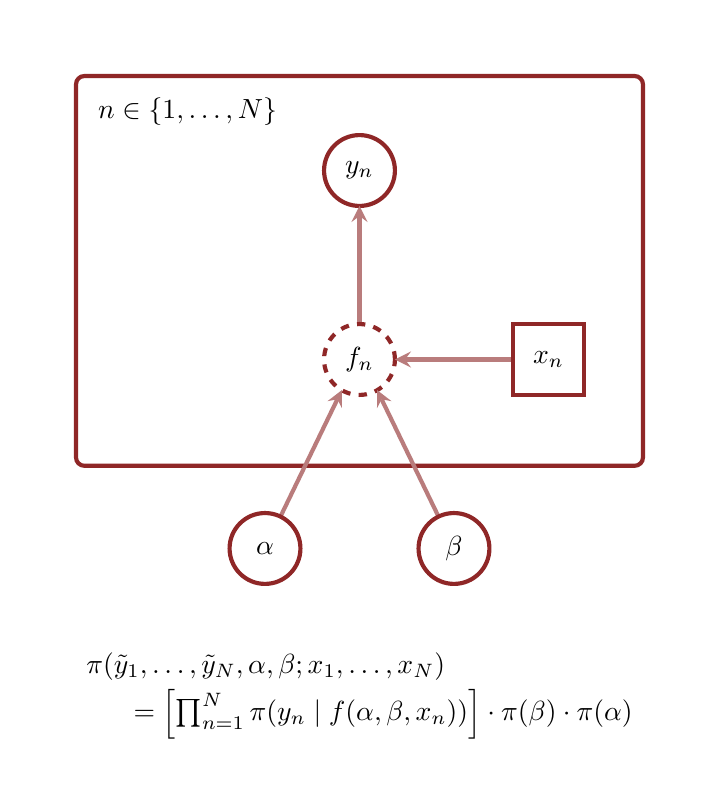
\begin{tikzpicture}[scale=0.3, thick]

\pgfmathsetmacro{\r}{1.5}

\pgfmathsetmacro{\dx}{0}
\pgfmathsetmacro{\dy}{0}

\draw[white] (-14 + \dx, -13 + \dy) rectangle (14 + \dx, 18 + \dy);

\filldraw[fill=white, draw=dark, line width=1.5, rounded corners=3pt] (-12 + \dx, -0.5 + \dy) rectangle (12 + \dx, 16 + \dy);

\node[right] at (-11.5 + \dx, 14.5 + \dy) { $n \in \{1, \ldots, N\}$ };

\filldraw[fill=white, draw=dark, line width=1.5] (0 + \dx, 12 + \dy) circle (\r)
node[color=black] { $y_{n}$ };

\draw[->, >=stealth, color=mid, line width=1.5] (0 + \dx, 4 + \dy) -- (0 + \dx, 12 - \r + \dy);

\filldraw[fill=white, draw=dark, dashed, line width=1.5] (0 + \dx, 4 + \dy) circle (\r)
node[color=black] { $f_{n}$ };

\draw[->, >=stealth, color=mid, line width=1.5] (8 + \dx, 4 + \dy) -- (0 + \r + \dx, 4 + \dy);

\filldraw[fill=white, draw=dark, line width=1.5] (8 - \r + \dx, 4 - \r + \dy) rectangle +(2 * \r, 2 * \r)
node[] at (8 + \dx, 4 + \dy) { $x_{n}$ };

\draw[->, >=stealth, color=mid, line width=1.5] (-4 + \dx, -4 + \dy) -- ({0 - \r * cos(60) + \dx}, {4 - \r * sin(60) + \dy});
\draw[->, >=stealth, color=mid, line width=1.5] (4 + \dx, -4 + \dy) -- ({0 + \r * cos(60) + \dx}, {4 - \r * sin(60) + \dy});

\filldraw[fill=white, draw=dark, line width=1.5] (-4 + \dx, -4 + \dy) circle (\r)
node[color=black] { $\alpha$ };

\filldraw[fill=white, draw=dark, line width=1.5] (4 + \dx, -4 + \dy) circle (\r)
node[color=black] { $\beta$ };

\node[right] at (-12 + \dx, -9 + \dy) {$\pi(\tilde{y}_{1}, \ldots, \tilde{y}_{N}, \alpha, \beta; x_{1}, \ldots, x_{N})$};

\node[right] at (-10 + \dx, -11 + \dy) {$= \left[ \prod_{n = 1}^{N} \pi(y_{n} \mid f(\alpha, \beta, x_{n}) ) \right] \cdot \pi(\beta) \cdot \pi(\alpha)$};

\end{tikzpicture}

\end{document}  